% XeLaTeX can use any Mac OS X font. See the setromanfont command below.
% Input to XeLaTeX is full Unicode, so Unicode characters can be typed directly into the source.

% The next lines tell TeXShop to typeset with xelatex, and to open and save the source with Unicode encoding.

%!TEX TS-program = xelatex
%!TEX encoding = UTF-8 Unicode

%%% Set Document Class, Font, and Geometry
\documentclass[12pt]{article}
\usepackage[margin=1in]{geometry}               % See geometry.pdf to learn the layout options. There are lots.
\geometry{
left=1in,
right=1in,
bindingoffset=0mm,
top=1in,
bottom=1in
}
\setlength{\parindent}{3em}
\setlength{\parskip}{0pt}
\renewcommand{\baselinestretch}{1.68}
\usepackage{fontspec,xltxtra,xunicode}
\defaultfontfeatures{Mapping=tex-text}	% Sets Times New Roman Fonts
\setromanfont[Scale=1.11,Mapping=tex-text]{Times New Roman}	% Sets Times New Roman Fonts
\setsansfont[Scale=MatchLowercase,Mapping=tex-text]{Times New Roman}	% Sets Times New Roman Fonts	
\setmonofont[Scale=MatchLowercase]{Times New Roman} 	% Sets Times New Roman Fonts
\usepackage{indentfirst}  % Indents the first paragraph after a section heading
\usepackage{pdflscape}
\usepackage{verbatimbox}

%%% Title Formatting
\usepackage{titlesec}
\titleformat*{\section}{\LARGE\bfseries}
\titleformat*{\subsection}{\normalfont \Large}{}
\titleformat*{\section}{\large\bfseries}
\titleformat*{\subsection}{\large\bfseries}
\titleformat*{\subsubsection}{\large\bfseries}
\titleformat*{\paragraph}{\large\bfseries}
\titleformat*{\subparagraph}{\large\bfseries}

%%% Drawing and Formatting
\usepackage{tikz}
\usepackage{pgfplots}
\usepackage{color}
\usepackage{graphicx}
\usepackage{amssymb}
\usepackage{float}
\restylefloat{table}
\edef\restoreparindent{\parindent=\the\parindent\relax}
\usepackage{parskip}
\restoreparindent
\pgfplotsset{compat=1.9}
\usepgfplotslibrary{fillbetween}
\usepackage{pgfplotstable}
%\usepackage{gnuplot}

%%% Bibliography Engine
\usepackage{harvard}
\bibliographystyle{agsm}
\citationstyle{agsm}


%%% Custom Headers and Footers Engine %%%
\usepackage{fancyhdr,lastpage}
\pagestyle{fancy}
\lhead{GVPT 392 (849)}
\chead{Mid-Term Exam}
\rhead{Nick Thompson}
\lfoot{}
\cfoot{\thepage}
\rfoot{}
\renewcommand{\headrulewidth}{.5pt}
\renewcommand{\footrulewidth}{.5pt}

%%% Table Engine %%%
\usepackage{booktabs,caption,fixltx2e}
\captionsetup[table]{labelfont=bf}
\newcommand{\ra}[1]{\renewcommand{\arraystretch}{#1}}
\usepackage[flushleft]{threeparttable}
\usepackage{multirow}
\usepackage{dcolumn}
\usepackage{rotating}

\title{GVPT 392 (849)}
\author{Nick Thompson}
\date{March 25, 2016}                                           % Activate to display a given date or no date

\begin{document}
%\maketitle

%%%%%%%%%%%%%%%%%%%     THIS BEGINS THE TITLE PAGE     %%%%%%%%%%%%%%%%%%%%%%%%
\begin{titlepage}
	
	\newcommand{\HRule}{\rule{\linewidth}{0.5mm}} % Defines a new command for the horizontal lines, change thickness here
	
	\center % Center everything on the page
	
	%----------------------------------------------------------------------------------------
	%	HEADING SECTIONS
	%----------------------------------------------------------------------------------------
	
	\textsc{\LARGE University of Maryland}\\[1.5cm] % Name of your university/college
	\textsc{\Large Department of Government and Politics}\\[0.5cm] % Major heading such as course name
	\textsc{\large GVPT - 392 (849):  Introduction to GIS for Social Science Research}\\[0.5cm] % Minor heading such as course title
	
	%----------------------------------------------------------------------------------------
	%	TITLE SECTION
	%----------------------------------------------------------------------------------------
	
	\HRule \\[0.4cm]
	{ \huge \bfseries Mid-Term Exam}\\[0.4cm] % Title of your document
	\HRule \\[1.5cm]
	
	%----------------------------------------------------------------------------------------
	%	AUTHOR SECTION
	%----------------------------------------------------------------------------------------
	
	\begin{minipage}{0.4\textwidth}
		\begin{flushleft} \large
			\emph{Author:}\\
			Nick \textsc{Thompson} % Your name
		\end{flushleft}
	\end{minipage}
	~
	\begin{minipage}{0.4\textwidth}
		\begin{flushright} \large
			\emph{Instructor:} \\
			Dr. James \textsc{Gimpel}\\ % Supervisor's Name
		\end{flushright}
	\end{minipage}\\[4cm]
	
	% If you don't want a supervisor, uncomment the two lines below and remove the section above
	%\Large \emph{Author:}\\
	%John \textsc{Smith}\\[3cm] % Your name
	
	%----------------------------------------------------------------------------------------
	%	DATE SECTION
	%----------------------------------------------------------------------------------------
	
	{\large October 5-7, 2016}\\ (extension granted to OCT 9 for illness)\\[3cm] % Date, change the \today to a set date if you want to be precise
	
	%----------------------------------------------------------------------------------------
	%	LOGO SECTION
	%----------------------------------------------------------------------------------------
	
	%\includegraphics{Logo}\\[1cm] % Include a department/university logo - this will require the graphicx package
	
	%----------------------------------------------------------------------------------------
	
	\vfill % Fill the rest of the page with whitespace
	
\end{titlepage}


%%%%%%%%%%%%%%%%%%%%%%%  THIS ENDS THE TITLE PAGE    %%%%%%%%%%%%%%%%%%%%%


The following coverages can be found in the PACD8 folder.

\begin{enumerate}
	\item PA\_CD8\_Voterfile: all registered voters for Pennsylvania, Congressional District 8.  This is north-suburban Philadelphia, including all of Bucks and part of Montgomery Counties.
	\item PA\_CD8\_Boundary: the outline for CD 8.
	\item PA\_and\_NJ\_Counties: County boundaries for the two states.
	\item Four\_States: State boundaries for PA, DE, NJ, and MD. %Rename Four\_States
	\item CD8\_PA\_Pct\_Data\_2012: voter precinct data for 2012.
	\item Mont\_County\_Recent\_Movers\_10\_12
	\item Bucks\_County\_Recent\_Movers\_10\_12
	\item CD8\_Places
	\item PA CD8\_Tracts
\end{enumerate}


\noindent Three files above contain points for voters at their residences.  These are 1, 6, and 7.  For these files, the following columns contain important information:

\noindent Age (and Year Born) = the age of the voter in 2012.

\noindent Rep\_Party, Dem\_Party, Ind\_Unaf\_Party = the party registration of the voter:  Rep = Republican, Dem = Democratic, and Ind\_Unaf = Independent/Unaffiliated.

\noindent And there are other items that will be less important for this exercise.
\\

\clearpage

For the following questions, use whatever tools you deem appropriate form the ArcGIS package, but be sure to describe what you did to address the questions.  Be resourceful, but you need not write more than one page in response to each question.


\noindent \textbf{1.  Aggregate the voter and mover data to the census tract level for PA CD8.}

To aggregate the data, I used a three phase process with multiple steps in each phase.  In Phase 1, I imported the data using the catalogue in ArcMap.  To import the data I first created a geodatabase file named \textbf{exam.gdb}.  Here I imported all exam shapefils included in the provided exam folder by right clicking on the \textbf{exam.gdb} and selecting import from multiple.  Next, I systemtaically added four file layers to the ArcMap table of contents:

\begin{itemize}
	\item PA\_CD8\_Voterfile (hereafter depicted as \textbf{voter}); 	
	\item Mont\_County\_Recent\_Movers\_10\_12 (hereafter depicted as \textbf{MC}); 	
	\item Buck\_County\_Recent\_Movers\_10\_12 (hereafter depicted as \textbf{BC});	
	\item PA\_CD8\_Tracts (hereafter depicted as \textbf{tracts}).  
\end{itemize}


This was the end of Phase 1. 

In Phase 2, I reviewed the data and deleted unnecessary fields.  The number is too great to depict which were removed.  I kept essential fields outlined in the instructions above, as well as some others that I anticipated would be necessary (including \textbf{MOVER} from the \textbf{voter} file, \textbf{ozipcode} and \textbf{dzipcode} from \textbf{MC} and \textbf{BC}, and \textbf{ORNIC}, \textbf{DRNIC}, and \textbf{RNIC} from \textbf{voter}, \textbf{BC}, and \textbf{MC}.  The combination of fields chosen allowed me to manipulate the data to achieve the desired results.  I removed fields by double-clicking on each layer in the table of contents and navigating to the \textbf{Fields} tab.  After clearing all of the fields, I was able to check only the fields I wanted to keep.  Next, I exported the data into new layers within the geodatabase.  This data management process ended Phase 2. 

In Phase 3, I used the \textbf{Spatial Join} feature (hereafter known as \textbf{SJ}) to systemtaically join the layers.  First I conducted a \textbf{SJ} of \textbf{vote\_total}voters\textbf{vote\_total} to \textbf{tracts} and created a new layer called \textbf{tracts01}.  Next I created the following \textbf{SJ}s: 

a.  \textbf{tracts} + \textbf{BC} = \textbf{tracts02} 

b.  \textbf{tracts} + \textbf{MC} = \textbf{tracts04} 

c.  \textbf{tracts01} + \textbf{tracts02} = \textbf{tracts03}

d.  \textbf{tracts03} + \textbf{tracts04} = \textbf{tracts07}

The last combination created a spatially joined dataset depicting the north-suburban part of Philadelphia.

\begin{itemize}
	\item Then compute and calculate the Democratic \% of total registered voters (10 points).
\end{itemize}

To calculate the percentage of total Democrat voters I went to the \textbf{voter} attribute table and selected the Democrat column.  I rigclicked.  That gave me the total number of Democrat voters ($203,185$).  I divided this number the total number of entries ($477,479$).  The outcome if that $42.55\%$ of people that voted Democrat in the database.

\begin{itemize}
	\item Compute and calculate the Democratic \% of total movers in Bucks and Montgomery counties (10 points).
\end{itemize}

To calculate the percentage of total Democrat voters from Bucks county I used the attribute table, right clicked on the Democrat field and copied the total number of Democratic voters ($22,555$).  Then I divided that by the total number of rows in the table ($48,923$).  This returns an output of $46.10\%$ of people voted Democratic in the Bucks movers county attribute table.

To calculate the percentage of total Democrat voters from Montgomery county I used the attribute table, right clicked on the Democrat field and copied the total number of Democratic voters ($2,016$).  Then I divided that by the total number of rows in the table ($5351$).  This returns an output of $37.67\%$ of people voted Democratic in the Montgomery movers county attribute table.

\begin{itemize}
	\item Produce two maps of these percentages. (20 points)
\end{itemize}

To produce my maps I followed some formatting guidelines.  First, I always included a legend, scale, and north seeking arrow.  Also included was my name as the author and the date I finalized the map.  

For this first set of maps I created two data layers.  In the first data layer I included the earlier aggregated data (\textbf{tract07}).  I included one each for Bucks and Montgomery counties.  This allowed me to produce a color ramp for each county's Democrat field normalized by total voters from the \textbf{voter} database. In the map this is depicted in the top map.  In the bottom map I normalized all Democratic voters against total voters using the same colorramp.    This depicts a strong concentration of Democratic voters located in the southeastern portion of the country. 

\begin{figure}
	\caption{Voting Distribution}
	\centerline{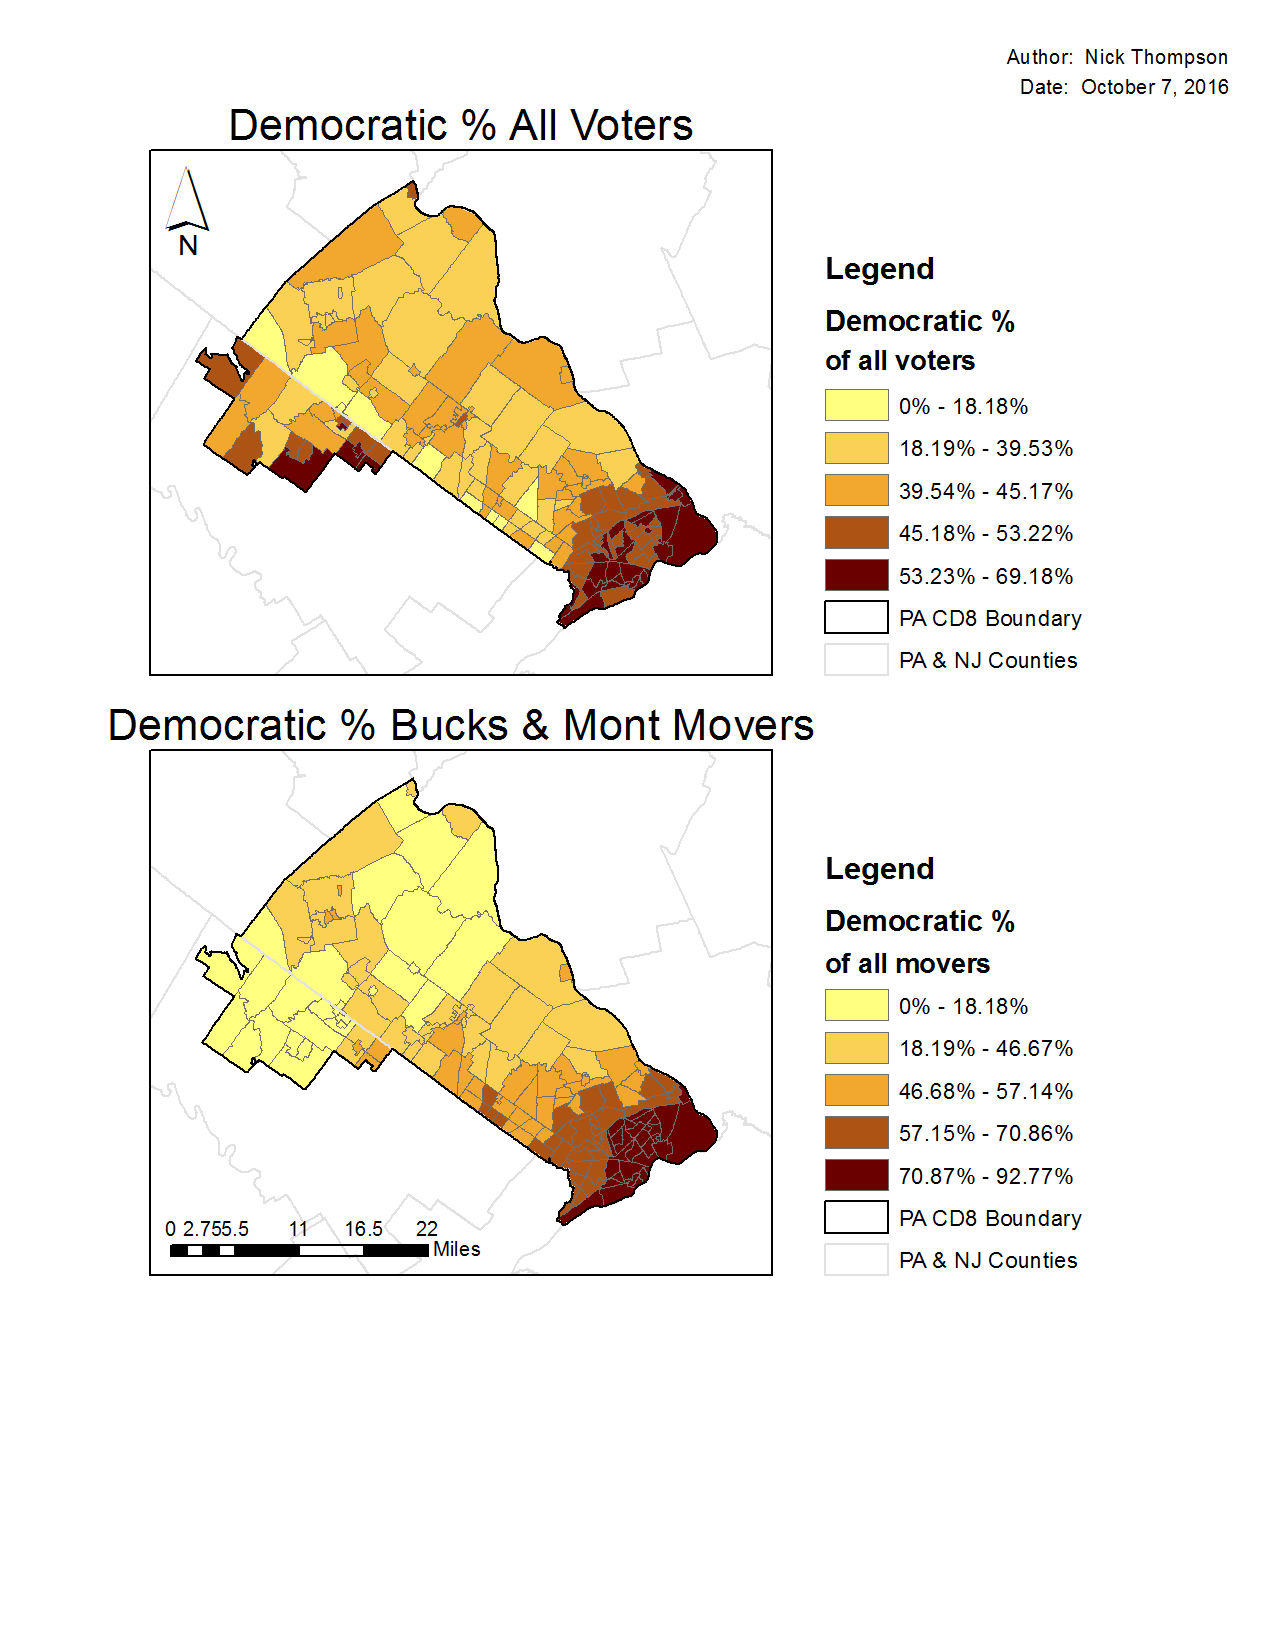
\includegraphics[scale=.75]{question_12.png}} % Figure 1:  Democratic Voters and Movers...
\end{figure}


\clearpage


\noindent \textbf{2. How would you characterize the spatial distribution of Republicans, Democrats, and Independents in PA CD8?  Write up two paragraphs based on what you have found, describing how you used ArcGIS to address the question.  (20 points)}

Figure 2 below shows how the parties are distributed in space.  To depict these figures I normalized the voterd data for each party according to the \textbf{voter} database against the \textbf{vote\_total} variable created above.  This produced three different spatial maps.   I utilized a five quantile break.  

Democrats tend to be located in the southeast, near the border with Philadelphia.  Republicans tend to be densely populated throughout the norther part of the districts, specifically Montgomery county and northern Bucks county.  Indepenedents tend to be distributed along the northern aspect of the southeastern portion of the district.
 
\begin{figure}[H]
	\caption{Parties in Space}
	\centerline{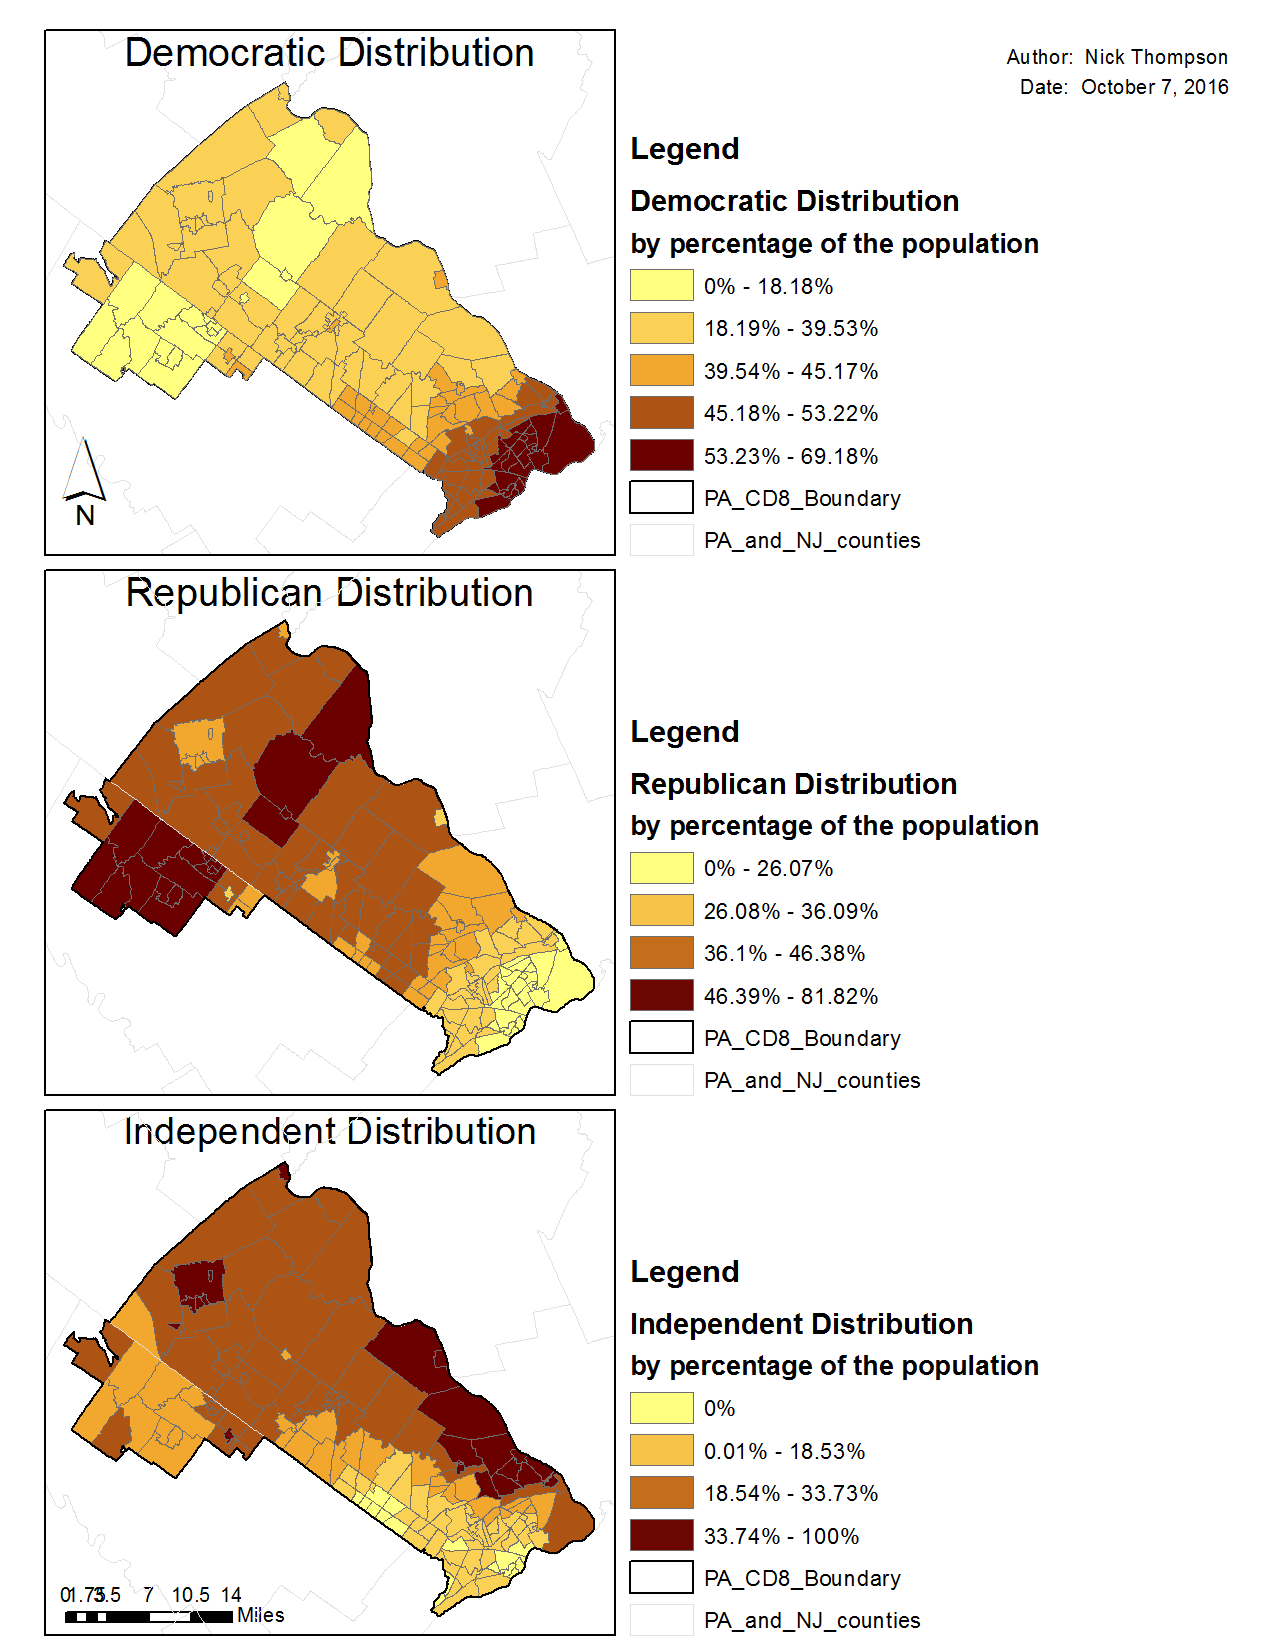
\includegraphics[scale=.75]{question_2.png}} % Figure 2:  Parties in Space
\end{figure}

\noindent \textbf{3.  The data included also show two populations of recent movers from inside PA and from nearby states.  How do the recent movers in Montogomery and Bucks counties compare by age and by party registration to the entire PA\_CD8 voting populations?  Explain your answer in no more than one page. (20 points)}

To answer this question I pulled the descriptive statistics for each dataset (\textbf{BC}, \textbf{MC}, \textbf{voter}) and collected the number of people that voted in each party, the party means, and the party standard deviations (Table 3).  I also collected the mean, standard deviation, minimum, and maximum values of the voters from each of the three datasets (Table 4).

The Montgomery county movers are represented by a higher percentage of Republicans than Democrats (Independents are behing Republicans and Democrats in all three datasets.  The Bucks county Democratic movers (46.10\%) have a significantly higher percentage than Montgomery county movers (37.68\%).  This indicates that either Democrats in Bucks county are migrating at higher rates, or that the percentage of voters in both counties falls around those means.

One way to differentiate between the two possibilities is to compare the means of the total voter population from the district.  If we assume a normal distribution of Republican, Democratic, and Independent voters throughout the district then the averages of 34.13\% for Republicans, 52.63\% for Democratic party voters, and 12.10\% for Independent voters should represent similar means the two counties.  

The Republican numbers in Bucks county are close to the overall voter mean, but the Montgomery mean is higher.  This indicates that Republicans are migrating to Montgomery county.  The mean of Democratic voters in both Bucks and Montgomery counties is significantly lower than in the \textbf{voter} database.  This may indicate less migration for Democratic voters.

The age demographics do not tell us as much without a geographic dispersion.  The mean and standard deviation of the three data sets is relatively similar, as depicted in Table 4.  As depicted in Figures 3-5, the age dispersion.  

In order to complete the maps I combined a choropleth map of each party (red for Repubulican, blue for Democrat, green for Independent) with a centroid map of the overall voting population.  This normalized the regiserted voters by each age group.  While the ages look identical in each map, the scales of the circles are different.  Note the low numbers of 18-29 year old voters in comparison to 30-49 year olds.

To create the centroid maps I followed this sequence.  First I created XY coordinate for each dataset by adding a new X and Y field respectively.  Next using the "Calculate Gemoetry" function for each X and Y respecitvely.  Next, I joined the \textbf{tracts} map with the \textbf{BC}, \textbf{MC}, and \textbf{voter} data sets.  Then I exported the joined tract datasets to a \textbf{vote\_total}tractCentroids\textbf{vote\_total} table.  This table now had the centroids for each voting block.  

To finalize the method I created a feature class from the XY \textbf{vote\_total}tractCentroids\textbf{vote\_total} table.  Opening the cataloge in ArcMap, I right clicked on \textbf{vote\_total}trackCentroids\textbf{vote\_total} and clicked "Create Feature Class" > "From XY Table".  I make the coordinate system the same as all of my other maps, the South Pennsylvania 1984.  Finally, I saved the file as a File and Personal Geodatabase called \textbf{vote\_total}voterTractCentroids\textbf{vote\_total}.


\begin{table}[]
\centering
\caption{Descriptive Statistics by Party}
\label{my-label}
\begin{tabular}{ccccc}
Dataset    & Party       & Vote Totals & Mean   & Std\\\_Dev \\ \hline
Montgomery & Republican  & 2230         & 0.4167 & 0.4930    \\
Montgomery & Democratic  & 2016         & 0.3768 & 0.4845   \\
Montgomery & Independent & 1043         & 0.1949 & 0.3962   \\ \hline
Bucks      & Republican  & 16808        & 0.3436 & 0.4748   \\
Bucks      & Democratic  & 22555        & 0.461  & 0.4984   \\
Bucks      & Independent & 8979         & 0.1835 & 0.3871   \\ \hline
Voter      & Republican  & 46085        & 0.3413 & 0.4742   \\
Voter      & Democratic  & 71048        & 0.5263 & 0.4993   \\
Voter      & Independent & 16334        & 0.121  & 0.3261  \\ \hline \hline
\end{tabular}
\end{table}


\begin{table}[]
\centering
\caption{Descriptive Statistics by Age}
\label{my-label}
\begin{tabular}{lllll}
\multicolumn{1}{c}{Data Set} & \multicolumn{1}{c}{Mean} & \multicolumn{1}{c}{\begin{tabular}[c]{@{}c@{}}Standard \\ Deviation\end{tabular}} & \multicolumn{1}{c}{Min} & \multicolumn{1}{c}{Max} \\ \hline
Montgomery                   & 43.81                    & 16.73                                                                             & 20                      & 104                     \\
Bucks                        & 44.83                    & 15.99                                                                             & 20                      & 104                     \\
Voter Data                   & 49.57                    & 17.50                                                                             & 0                       & 112                    \\ 
\hline 
\hline
\end{tabular}
\end{table}

\clearpage

\noindent \textbf{4.  Are movers more likely to relocate to particular locations than the general voter populations within PA CD8?  Or are they geoographically distributed about the same way?  Explain what you find in no more than one page.}

To calculate this I used the \textbf{tract07} again.  This time I aligend the democratic voters from each county database and compared it to the total voter database.  The Bucks and Montgomery spatial densities are normalized over the total voter population.  This gives me an understanding of the density with relation to all voters.  The normalization allows an analysis of migration patterns.  Said differently, comparing the two mover counties against the total population allows me to visualize migration patterns.

Republicans tend to be densely located in the north easter portion of Bucks county and generally dispersed in Montgomery county.  This seems to hold with previous depictions.  This indicated people tend to move to these areas.

Republicans movers in Bucks county tended to move to the north eastern part of the county.  Under a total voter proportion Republicans were densly populated in the northwester portion of the county.  Under a Bucks county movers proportion of voters Republicans were more densly populated in the northeastern part of the county.  

Democrats are heavily located in the southeastern portion of Buck and the total voter population, with a very sparse population in the north of Bucks county.  This indicates that these voters don't migrate as much as the republican voters. Democrats appear to migrate to similar areas as Republicans in Montgomery county. 

Independents tend to be widely dispersed, indicating they don't migrate much.

\begin{figure}[H]
	\caption{Republicans}
	\centerline{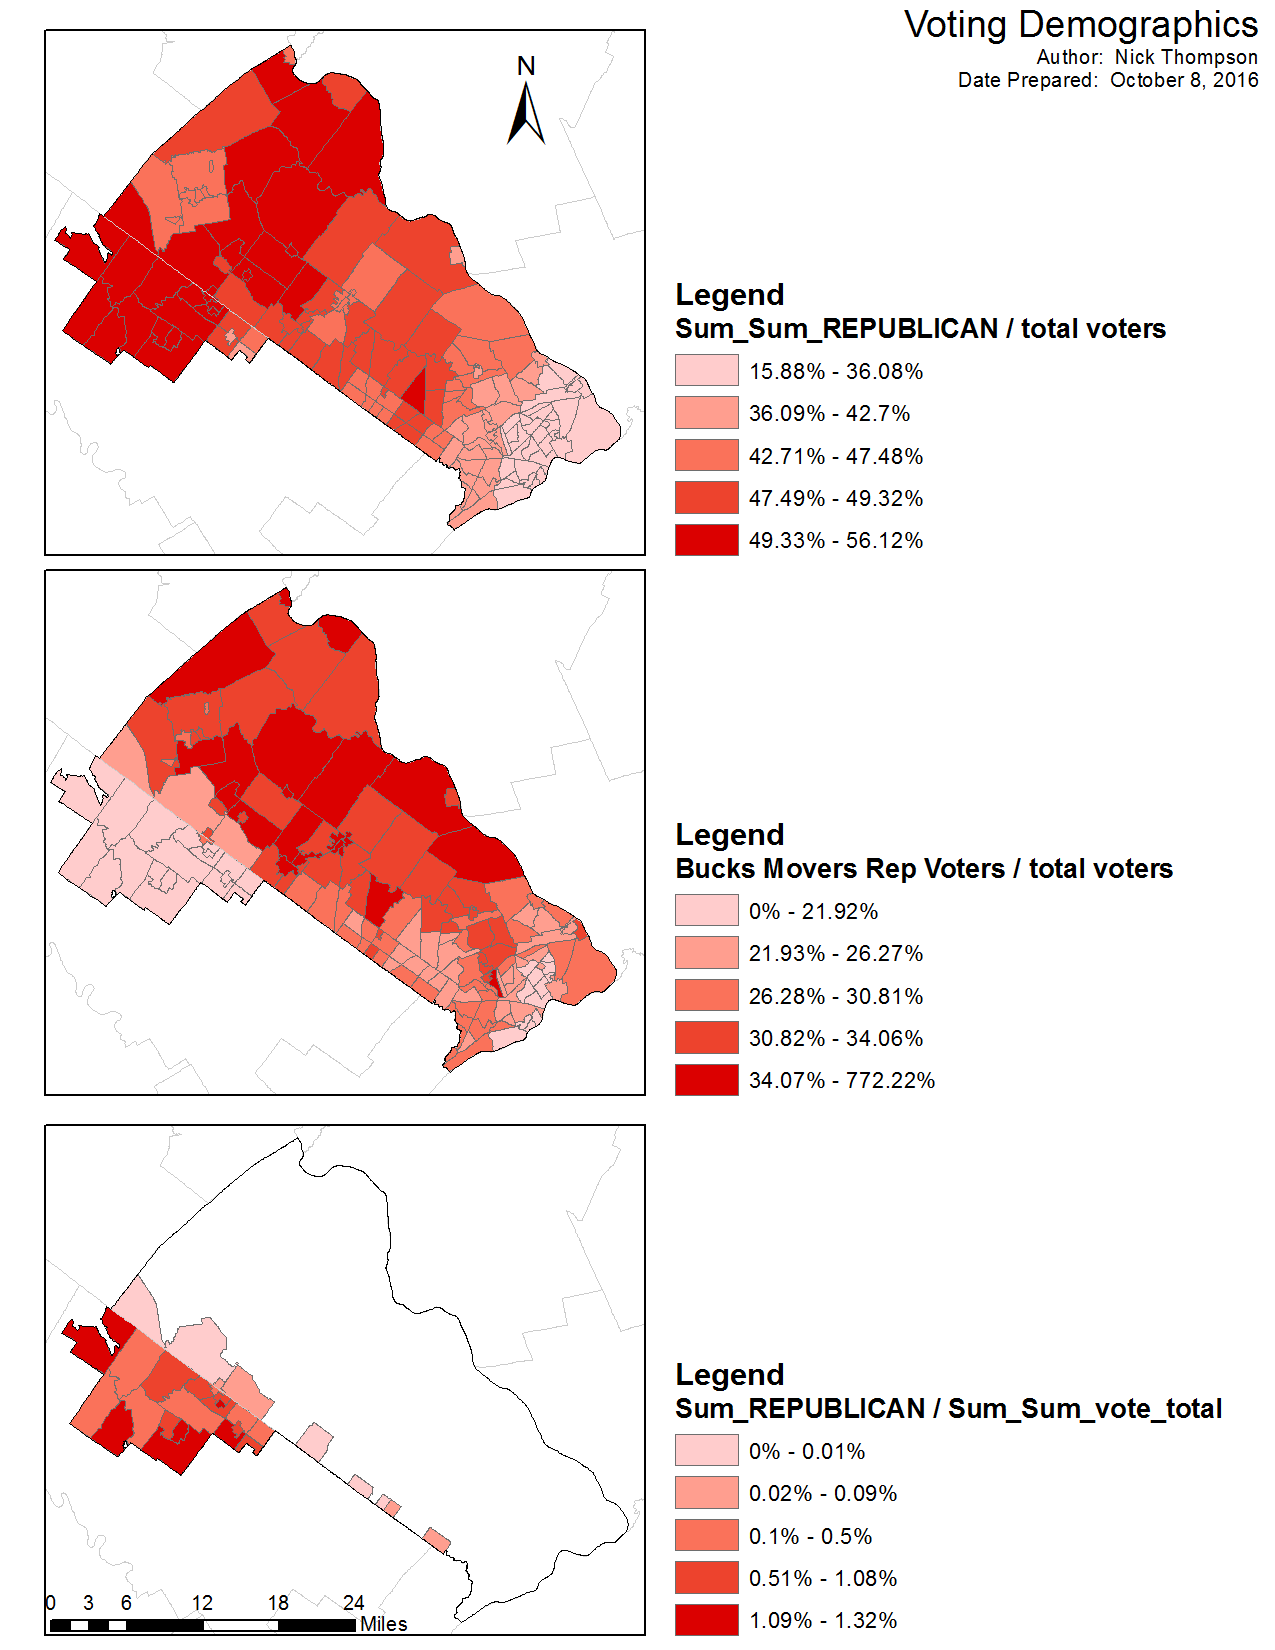
\includegraphics[scale=.75]{question_4a.png}} % Figure 3:  republican movers and voters
\end{figure}

\clearpage

\begin{figure}
	\caption{Democrats}
	\centerline{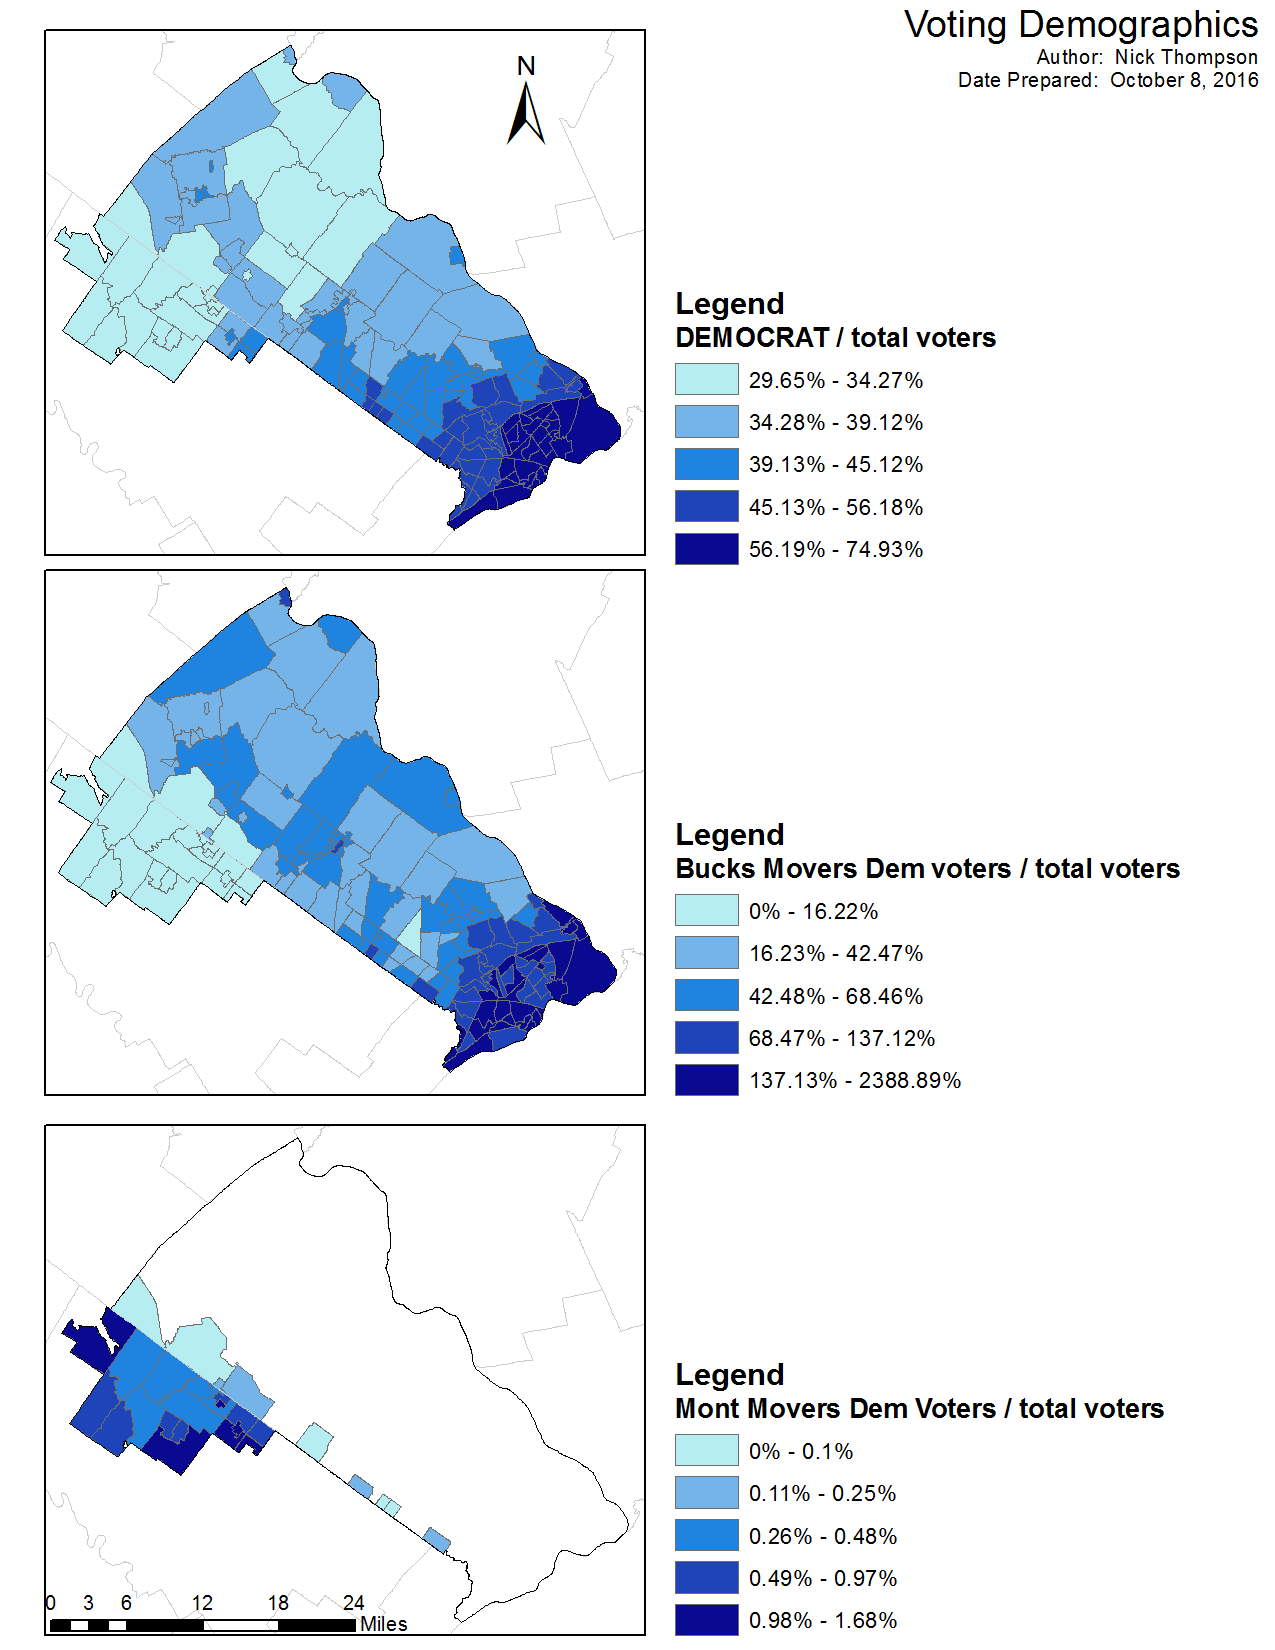
\includegraphics[scale=.75]{question_4b.png}} % Figure 4:  dem movers and voters
\end{figure}

\clearpage

\begin{figure}
	\caption{Independents}
	\centerline{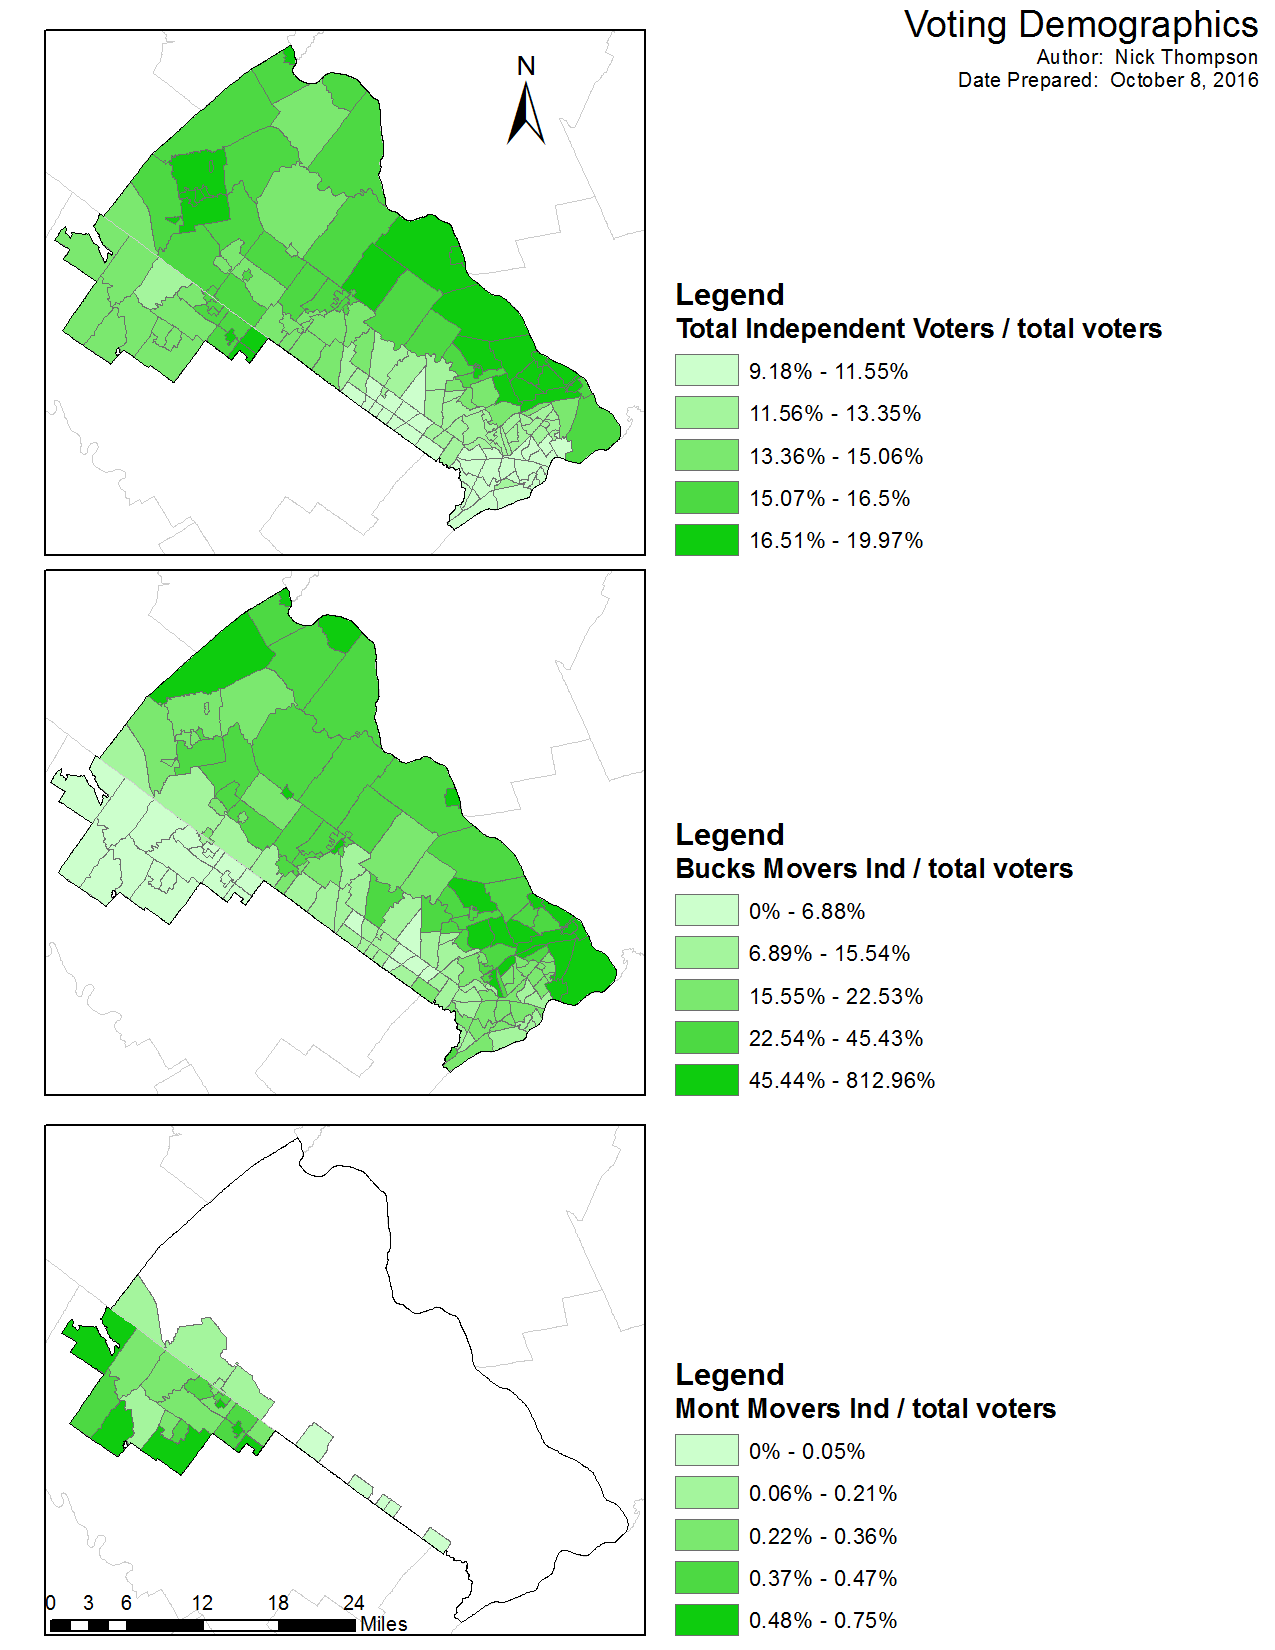
\includegraphics[scale=.75]{question_4c.png}} % Figure 5:  ind movers and voters
\end{figure}

\clearpage	

\noindent \textbf{5.  How many Bucks County voters live within one half-mile of the border with Philadelphia?  (10 points)}

To answer questions $5$, $6$, and $7$ I used the following processes and steps.  Noted differences are discussed in each question, but generally a process or step for questions $6$ and $7$ follow described processes or steps described in the following discussion.

There are $10,318$ voters in Bucks County within one half of a mile of the border with Philadelphia.  I found this information through the following process:

\begin{enumerate}
	\item Step 1:  Identify data to use:
	\begin{enumerate}
		\item The \textbf{voters} dataset and the \textbf{PA\_and\_NJ\_counties} dataset.  I used the attribute tables from each.  A single entry in the \textbf{PA\_and\_NJ\_counties} dataset identifies the boundary of Philadelphia (object ID \#72).  To find this quickly and select it I sorted ascending the \textbf{City\_Boundary} field and scrolled to the one indicating Philadelphia.
	\end{enumerate}
	\item Step 2:  I needed to isolate the Bucks county voters within the \textbf{voters} dataset.  I opened the attribute table and identified the field I needed to use (\textbf{JURISNAME}).  Selecting by attribute, from the selection menue, I chose the \textbf{voter} layer > Method: create new selection > double click \textbf{JURISNAME} > $=$ > "Get Unique Values" > double click \textbf{Bucks County} > Apply > Ok.
	\begin{enumerate}
		\item Next I exported the selected features to a new \textbf{vote\_total} File and Personal Geodatabase Feature Class\textbf{vote\_total} called \textbf{Voter\_BucksCty} > Export Data > Selected Records > Output Table.  Next I went to the catalog and put the new \textbf{Voter\_BucksCty} into the Table of Contents.
	\end{enumerate}
	\item Step 3:  To identify the voters within a half of a mile (0.5 miles), I "Select by Location" from the "Selection" menu.  
	\begin{enumerate}
		\item Select only \textbf{Voter\_BucksCty} layer in the "Target Layers" dialogue box > Selection method:  "Select from Features" > Source layer:  \textbf{PA\_and\_NJ\_counties} (with Philadelphia selected as noted above) > Spatial selection method for target features:  "are within a distance of the source layer feature" > distance = 0.5 > unit of measure:  "miles".
	\end{enumerate}
	\item Step 4:  Open the \textbf{Voter\_BucksCty} attribute table and "show selected records".  At the bottom there are two numbers:  10,318 records selected of 425,956 total records.
\end{enumerate}

\noindent \textbf{6.  How many Bucks County voters live within one mile of the border with Philadelphia?  (10 points)}

There are $17,206$ voters in Bucks County within one mile of Philadelphia.

To answer this question I already had the base processes and layers compiled.  To change the distance I returned to "Selection" > "Select by Location".  I kept all of the information the same, but I changed the distance from $0.5$ miles to ($1.0$) miles.  Next, I returned to the \textbf{Voter\_BucksCty} attribute table and recorded the new calculated numbers:  $17,206$ records selected of $425,956$ total records.

\noindent \textbf{7.  What percentage are those two figures of the total Bucks County voter population?}

To answer this question I have all of the data I need from the previous questions.  Arithmatic reveals the answer:  

\begin{itemize}
	\item Voters residing within $\frac{1}{2}$ mile:  $\frac{10,318}{425,956} = 0.0242$, or $2.42\%$
	\item Voters residing within 1 mile:  $\frac{17,206}{425,956} = 0.0404$, or $4.04\%$
\end{itemize}

%%%%%%%%%%%%%%%%%%%%%%White Board%%%%%%%%%%%%%%%%%%%%%%%%
\iffalse





\fi
%%%%%%%%%%%%%%%%%%%%%%%%%%%%%%%%%%%%%%%%%%%%%%%%%%%%
\clearpage
\bibliography{/Users/Nick/Documents/Library/Citations/mylibrary.bib}
\end{document}